%% Los cap'itulos inician con \chapter{T'itulo}, estos aparecen numerados y
%% se incluyen en el 'indice general.
%%
%% Recuerda que aqu'i ya puedes escribir acentos como: 'a, 'e, 'i, etc.
%% La letra n con tilde es: 'n.

\chapter{Introducci\'on}
\label{Chapter1} % Change X to a consecutive number; for referencing this chapter elsewhere, use \ref{ChapterX}

%----------------------------------------------------------------------------------------
%	SECTION 1
%----------------------------------------------------------------------------------------

\section{Hidrogeles polim\'ericos: Aplicaciones biomedicas.} 

%%%%%%%%%%%%%%%%%%%%%%%%%%%%%%%%%%%%%%%%%
En la \'ultima d\'ecada, el inter\'es por los hidrogeles polim\'ericos ha aumentado significativamente, debido a la amplia variedad y diversidad de materiales e innovaciones que se pueden lograr con ellos. Estos sistemas polim\'ericos, que tienen una estructura molecular flexible y adaptable, pueden alterar su forma y propiedades de acuerdo con las condiciones externas.
Esta adaptabilidad los convierte en protagonistas indispensables en diversas industrias \cite{zhu2022review}, desde su uso en la creaci\'on de espumas y adhesivos \cite{wu2021review, chowdhury2019novel}, hasta su aplicaci\'on en la industria cosm\'etica y de pinturas, ofreciendo caracter\'isticas singulares a productos que enriquecen nuestra vida diaria \cite{hirst2019fundamentals}.
En la industria alimentaria, los hidrogeles polim\'ericos act\'uan como aditivos esenciales, contribuyendo a la textura, preservaci\'on y seguridad de los alimentos que consumimos \cite{kwok2019microgel}.

Los hidrogeles se pueden utilizar para mejorar la retenci\'on de agua y nutrientes en el suelo, lo que puede ayudar a aumentar la productividad de los cultivos y reducir la necesidad de riego \cite{el2004radiation}. Adem\'as, estos materiales se pueden utilizar para proteger las plantas de las sequ\'ias y las plagas.
En el \'ambito de la remediaci\'on ambiental, los hidrogeles se pueden utilizar para adsorber y retener contaminantes \cite{perez2018using,perez2019molecular}, lo que puede ayudar a limpiar el agua, el suelo y el aire. Adem\'as, los hidrogeles se pueden utilizar para transportar y liberar agentes remediadores, acelerando el proceso de limpieza \cite{mehrotra2021use}.
En general, los hidrogeles polim\'ericos son materiales vers\'atiles con un amplio potencial de aplicaci\'on. Su capacidad para adaptarse a diferentes condiciones los convierte en una herramienta valiosa para una variedad de industrias.

Sin embargo, uno de los terrenos m\'as emocionantes en los que los hidrogeles polim\'ericos han causado un impacto significativo es en el \'ambito m\'edico y farmac\'eutico. Estos materiales se han erigido como protagonistas en la b\'usqueda de transportadores de f\'armacos m\'as avanzados, eficientes, amigables con el ambiente y compatibles con el organismo humano. Sus propiedades intr\'insecas les permiten ser moldeados y adaptados de manera espec\'ifica para cumplir con los requisitos \'unicos de la administraci\'on de medicamentos.
Esta capacidad permite dise\~nar hidrogeles personalizados que se adapten a las necesidades espec\'ificas de cada paciente.
Esta intersecci\'on entre los hidrogeles polim\'ericos y la medicina no solo tiene el potencial de revolucionar la forma en que entregamos y administramos medicamentos, sino que tambi\'en puede tener un impacto positivo en la calidad de vida de las personas. Tratamientos m\'as efectivos y personalizados que minimizan los efectos secundarios, gracias a la capacidad de estos materiales para interactuar de manera selectiva con el cuerpo humano. Adem\'as, la biodegradabilidad de estos materiales contribuye a la reducci\'on del impacto ambiental, lo que es fundamental en un mundo cada vez m\'as enfocado en la sostenibilidad.
La biodegradabilidad de los hidrogeles permite que se eliminen del cuerpo de manera natural, evitando la necesidad de cirug\'ias para su extracci\'on.

En estas \'ultimas aplicaciones m\'edicas, en particular, los films y micro/nanogeles polim\'ericos han sido pioneros en su uso y han tenido un creciente inter\'es.
Los films y geles polim\'ericos son materiales que han sido ampliamente estudiados y utilizados en diversas aplicaciones, incluyendo la medicina.
Estos materiales se forman por la uni\'on de cadenas largas de mol\'eculas org\'anicas, es decir pol\'imeros, que pueden tener diferentes grados de entrecruzamiento y solvataci\'on. En la figura \ref{fig:intro:acidos-aa-maa} se ilustra c\'omo a partir de una cadena polim\'erica es posible crear una red de la misma y as\'i obtener un film o micro/nanogel. Estos pol\'imeros est\'an compuestos por mon\'omeros que son quienes les dan cualidades extraordinarias y son las responsables de sus m\'ultiples aplicaciones.

Los films polim\'ericos son capas delgadas y planas de material polim\'erico que pueden tener diferentes espesores. Mientras que los microgeles son part\'iculas tridimensionales de pol\'imeros entrecruzados que, al igual que los films, tienen la capacidad de adsorber grandes cantidades de agua o solventes. Los nanogeles son estructuras similares a los microgeles, pero su tama\~no se encuentra en la escala nanom\'etrica.


Los films y geles polim\'ericos tienen la ventaja de poder modificarlos y manipularlos, lo que les permite adaptarse a diferentes necesidades y funciones.
Como resultado, los hidrogeles de pol\'imeros son actualmente candidatos prometedores para el desarrollo de una variedad de biomateriales con aplicaciones en biosensores \cite{zhang2012ultrathin,islam2014responsive}, ingenier\'ia de tejidos \cite{matricardi2013interpenetrating,van2011biopolymer}, regeneraci\'on \'osea \cite{bai2018bioactive}, materiales biomim\'eticos \cite{green2016mimicking,wu2010multifunctional}, entre muchas otras aplicaciones biom\'edicas \cite{Daly2020}.
Por ejemplo, los hidrogeles se pueden utilizar para crear parches transd\'ermicos que liberen f\'armacos de manera controlada y sostenida \addcite.

En conclusi\'on, hidrogeles polim\'ericos tienen un gran potencial para revolucionar una amplia gama de industrias, desde la cosm\'etica y alimentaria hasta la medicina y la farmac\'eutica. Su capacidad de adaptarse a diferentes condiciones y necesidades los convierte en una herramienta vers\'atil y valiosa para el desarrollo de nuevos productos y aplicaciones.



%%%%%%%%%%%%%%%%%%%%%%%%%%%%%%%

\section{Motivaci\'on...Encapsulado y Liberaci\'on de medicamentos}
%%%%%%%%%%%%%%%%%
%%%%hablar de los componentes de la red polimerica
%%%%porque se usan estos monomeros ???
%%%%%%%%%%%%%%%%%

La respuesta a est\'imulos de los films y/o micro/nanogeles est\'a fuertemente ligada a la composici\'on de los pol\'imeros que forman parte de su red tridimensional.
Los hidrogeles compuestos por cadenas polim\'ericas que contienen segmentos \'acidos como el \'acido acr\'ilico o metacr\'ilico (AA y MAA, respectivamente), suelen hincharse o deshincharse en respuesta a cambios en el pH de la soluci\'on en la que se encuentran \cite{snowden1996colloidal}.
Esta respuesta al pH viene acompa\~nada con una regulaci\'on de carga, con lo que se percibe en la mayor\'ia de los casos una respuesta a la concentraci\'on salina \cite{longo2019protonation}.
An\'alogamente, los hidrogeles compuestos por cadenas de pol\'imeros termosensibles experimentan una transici\'on de fase de volumen. Esta respuesta viene caracterizada por una temperatura caracter\'istica \cite{Pelton1986,Pelton2000}.
Este comportamiento se origina porque tales pol\'imeros son insolubles en agua por encima de cierta temperatura de soluci\'on cr\'itica m\'as baja (LCST por sus siglas en ingl\'es) \cite{Kawaguchi2020}.
En particular, los hidrogeles compuestos por poli(N-isopropilacrilamida) (PNIPAm) poseen una LCST de alrededor de 32$^\circ$C \cite{Schild1992}.

En la figura \ref{fig:intro:acidos-aa-maa} se muestran los diferentes mon\'omeros que pueden contener las cadenas polim\'ericas que componen la red de los nanogeles. Los primeros tres muestran respuesta al pH y a la concentraci\'on salina (alilamina, \'acido metacr\'ilico y \'acido acr\'ilico), la \'ultima mol\'ecula es la N-isopropilacrilamida (NIPAm) la cual presenta respuesta a la temperatura.


\begin{figure*}[!tb]
	\centering
	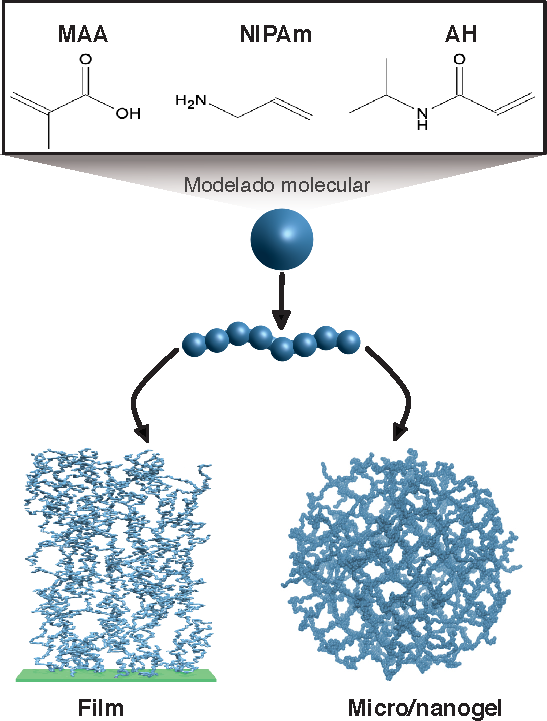
\includegraphics[width=0.75\linewidth]{Figures/modelos/hidrogeles.pdf}
	\caption{Mol\'eculas  que conforman los diferentes mon\'omeros de las redes polim\'ericas que dan respuesta a los hidrogeles que se abordan en esta tesis. Con respuesta al pH y concentraci\'on de sal: alilamina (AH) y  \'acido metacr\'ilico (MAA). con respuesta a la temperatura: N-isopropilacrilamida (NIPAm).}
	\label{fig:intro:acidos-aa-maa}
\end{figure*}

Los mon\'omeros presentados en la figura \ref{fig:intro:acidos-aa-maa} tienen la particularidad de formar redes tridimensionales biodegradables y biocompatibles \cite{bajpai2008responsive}, lo que los vuelve atractivos para el dise\~no de biomateriales.
Adem\'as, el mon\'omero del pol\'imero termosensible, NIPAm, al poseer una temperatura de transici\'on de volumen alrededor de la temperatura corporal, sus hidrogeles han generado un gran inter\'es para aplicaciones biom\'edicas \cite{Guan2011}.

Es posible conseguir estrategias para controlar la temperatura de transici\'on de estos hidrogeles, las cuales incluyen la copolimerizaci\'on con un mon\'omero i\'onico o ionizable \cite{Cai2007,Macchione2019, Hirose1987,Lopez2020}.
Este \'ultimo enfoque produce hidrogeles de respuesta m\'ultiple que son susceptibles a cambios en la temperatura, el pH y la concentraci\'on de sal.
Los microgeles de NIPAm y AA han sido ampliamente estudiados, y se ha demostrado que su temperatura de transici\'on depende del pH de la soluci\'on y la concentraci\'on de sal \cite{Morris1997, Jones2000,Bradley2005,Begum2016}.
Tambi\'en se han investigado microgeles de copol\'imeros de NIPAm y MAA \cite{Dowding2000,Hoare2004,Giussi2015}, y se ha demostrado que su temperatura de transici\'on tambi\'en depende de la fracci\'on de mon\'omero ionizable en las cadenas de pol\'imero \cite{Morris1997,Jones2000, Hoare2004, Bradley2005, Lee2008,Wong2009,Hamzavi2016}.


%%%%%%%%%%%%%%%%%%%%%
%%%% aquí va el encapsulado
%%%%%%%%%%%%%%%%%%
La naturaleza hidrof\'ilica de los nanogeles son generalmente biocompatibles y poseen una gran capacidad para incorporar mol\'eculas hu\'esped o analitos, tanto org\'anicos como inorg\'anicos, y prevenir su degradaci\'on por el medio externo.
El ambiente acuoso dentro de los hidrogeles puede proteger a las prote\'inas de la desnaturalizaci\'on y la agregaci\'on durante cuando se liberan de los hidrogeles \cite{asayama2008comparison,sawada2010nano,beierle2014polymer}, mientras permanecen activas y estructuradas cuando se liberan de los hidrogeles \cite{vermonden2012hydrogels}.
En la administraci\'on oral de f\'armacos, los hidrogeles con respuesta de pH se han investigado en gran medida como veh\'iculos funcionales que pueden encapsular y administrar prote\'inas, evitando su degradaci\'on por el entorno gastrointestinal \cite{malmsten2010biomacromolecules,renukuntla2013approaches,koetting2014ph}.
Adem\'as, su escaso tama\~no les permite responder r\'apidamente luego de recibir el est\'imulo \cite{tanaka1979kinetics}.



%%%
%%explicar el esquema 
Nanogeles con respuesta al pH se han considerado para la administraci\'on oral de f\'armacos. En este \'ambito, los cambios de pH que ocurren a lo largo del tracto digestivo, desde un medio \'acido en el est\'omago (pH 1.2-2) hasta uno neutro o moderadamente alcalino en el intestino delgado (pH 7-8), pueden ser aprovechados para controlar la liberaci\'on de f\'armacos.
Adem\'as, algunos compartimentos celulares involucrados en la captaci\'on de f\'armacos, como los endosomas tempranos, tienen un pH levemente \'acido. La diferencia de pH que existe entre la superficie de la piel y el torrente sangu\'ineo puede ser aprovechada para la administraci\'on transd\'ermica de f\'armacos utilizando nanogeles con respuesta al pH \cite{qindeel2019development}.
Esto se ve esquematizado en la figura \ref{fig:intro:sistema} en la cual se muestra c\'omo la respuesta a est\'imulo, pH, temperatura, concentraci\'on de sal,  de los nanogeles funciona como agente liberador de drogas ya sea por un colapso o expansi\'on de la part\'icula (lado izquierdo).
A la derecha de la figura, se muestran los diferentes ambientes del tracto digestivo, en cuanto a valores de pH, con los cuales se pueden aprovechar los nanogeles con respuesta al pH.


\begin{figure}
	\centering
	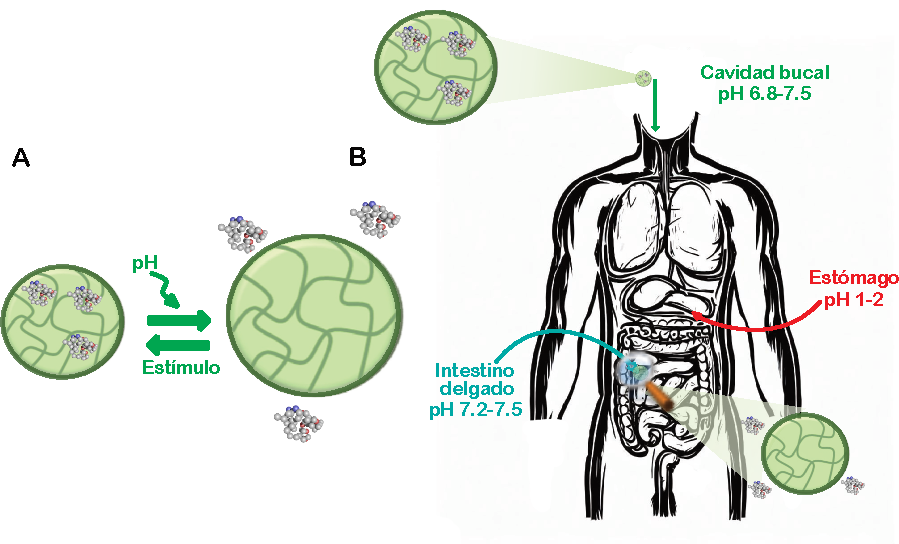
\includegraphics[width=0.99\textwidth]{Figures/modelos/sistema.pdf}
	\caption{Esquema de funcionamiento de nanogeles como transportadores de medicamentos. 
		\textbf{A} (izquierda): nanogel cargado con una prote\'ina terap\'eutica que la libera por respuesta a un est\'imulo. \textbf{B} (lado derecho)Se aprovecha los diferentes ambientes que hay en el cuerpo humano para el dise\~no de nanogeles que liberen drogas terap\'euticas en un ambiente espec\'ifico. }
	\label{fig:intro:sistema}
\end{figure}

Por otro lado, el microambiente local alrededor del tejido canceroso puede presentar un pH m\'as \'acido en comparaci\'on con las condiciones fisiol\'ogicas habituales \cite{lawson1963breast,tannock1989acid,gerweck2006tumor}, por lo que los nanogeles con respuesta al pH est\'an siendo evaluados para la administraci\'on de medicamentos en el tratamiento del c\'ancer en el futuro \cite{peng2013controlled,kanamala2016mechanisms}. Por ejemplo, se han utilizado nanogeles de quitina para la administraci\'on de doxorubicina en diferentes tipos de c\'ancer, incluyendo pulm\'on, mama, h\'igado y pr\'ostata \cite{jayakumar2012doxorubicin}.

Por otro lado, los nanogeles de pol\'imeros termosensibles pueden ser utilizados para la administraci\'on localizada de anest\'esicos \cite{indulekha2016thermoresponsive} . Como veh\'iculos para el suministro de drogas, los nanogeles polim\'ericos pueden administrar f\'armacos de peso molecular bajo, oligonucle\'otidos, prote\'inas terap\'euticas e incluso combinaciones de drogas, lo cual es esencial en terapias contra el c\'ancer y las enfermedades infecciosas.

Recientemente se investigaron dispositivos basados en microgeles de poli(NIPAm-co-MAA) para la encapsulaci\'on/liberaci\'on del f\'armaco quimioterap\'eutico Doxorrubicina \cite{Giussi2020, MartinezMoro2020, Pergushov2020}. Estos autores mostraron el uso de microgeles para la liberaci\'on controlada de sustancias bioactivas con carga opuesta.
La incorporaci\'on del comon\'omero \'acido proporciona un mecanismo controlado por el pH para la captura/liberaci\'on de mol\'eculas con carga opuesta, lo que hace que los microgeles de respuesta múltiple sean atractivos para el dise\~no de sistemas funcionales de administraci\'on de f\'armacos \cite{Liu2017}.

%%%%%%%%
En s\'intesis, el rango de las potenciales aplicaciones biom\'edicas de los nanogeles es extenso e incluye desarrollos, m\'as espec\'ificamente en medicina, contra los trastornos neurol\'ogicos, las enfermedades cardiovasculares, oftalmol\'ogicas, inflamatorias y autoinmunes, as\'i como tambi\'en avances en el diagn\'ostico por im\'agenes, la ingenier\'ia de tejidos, la reconstrucci\'on \'osea y el manejo de la diabetes y el dolor. Por ejemplo, los nanogeles de \'acido hialur\'onico est\'an siendo evaluados para inhibir la acumulaci\'on de la prote\'ina beta-amiloide en el manejo del Alzheimer \cite{jiang2018nanogels}. En el tratamiento de la diabetes, se investigan nanogeles sensibles a la glucosa \cite{wu2010multifunctional} y nuevos m\'etodos de administraci\'on de insulina basados en nanogeles \cite{nolan2004thermally}.

Estas son algunas razones por las cuales los nanogeles polim\'ericos son hoy en d\'ia una de las primeras opciones consideradas al dise\~nar biomateriales con funciones espec\'ificas \cite{soni2016nanogels,sabir2019polymeric}. El est\'imulo que dispara la respuesta de los nanogeles puede ser suministrado por un gradiente en la composici\'on fisiol\'ogica, ya sea natural o inducido por un estado patol\'ogico. La versatilidad de estos materiales dif\'icilmente puede ser alcanzada con otro tipo de nanopart\'iculas, incapaces de responder a cambios en las condiciones del medio que pueden ser relativamente moderados.

Uno de los desaf\'ios en la actualidad es aprender a controlar esta respuesta para canalizarla en diferentes aplicaciones. A lo largo de esta tesis se plantea dicho desaf\'io de tal manera de comprender la fisicoqu\'imica, relevante,  que involucra a los hidrogeles polim\'ericos, films y micro/nanogeles, con su capacidad de responder a est\'imulos y como consecuencia ser utilizados para el desarrollo de dispositivos para el encapsulado y liberaci\'on de medicamentos.

En la siguiente secci\'on se plantean los objetivos de la tesis en el marco de lo desarrollado en la misma.


\section{Objetivos}

En la b\'usqueda de estudiar el uso de los hidrogeles polim\'ericos como transportadores de medicamentos, se plantearon diferentes objetivos de tal forma de comprender la fisicoqu\'imica que envuelve a todos estos sistemas.

En primera instancia, en el cap\'itulo \ref{Chapter-film}, se estudi\'o y se muestra el uso de films polim\'ericos basados en \'acido poli(metacr\'ilato) (PMAA) como capturadores de poliaminas, las cuales funcionan como disparadores para la liberaci\'on de doxorubicina. En este trabajo se \textbf{desarroll\'o un modelo mecano-estad\'istico utilizando Teor\'ia Molecular (TM)} para describir la respuesta a cambios de pH y concentraci\'on de sal.

En el cap\'itulo \ref{Chapter-geles}, se incorporaron co-mon\'omeros de NIPAm de modo \textbf{de extender dicho modelo para investigar el comportamiento de microgeles de copol\'imeros con respuesta a m\'iltiples est\'imulos}. En particular se estudiaron microgeles polim\'ericos compuestos por poli-(NIPAM-co-MAA) que poseen respuesta multi-est\'imulo (pH, concentraci\'on salina y temperatura) y su potencial uso como encapsuladores de drogas anti-cancer\'igenas como la daunorubicina y la doxorubicina.
Para dicho estudio se deriv\'o una nueva teor\'ia termodin\'amica que permit\'ia el estudio de estos microgeles considerandolos como una fase homog\'enea.

En el cap\'itulo \ref{Chapter-esfericas} se estudiaron \textbf{los mecanismos de adsorci\'on de diferentes biomol\'eculas en los microgeles en funci\'on de las condiciones del medio y la estructura/composici\'on qu\'imica de las cadenas polim\'ericas}. Los nanogeles basados en MAA y AH son utilizados para comprender c\'omo la estructura de la red polim\'erica modifica la adsorci\'on de prote\'inas como lo son el citocromo c, mioglobina y la insulina.

En este cap\'itulo se \textbf{combinaron simulaciones de TM y Din\'amica Molecular (DM)}, esta \'ultima para la obtenci\'on de las configuraciones que dan origen a las estructuras de las redes polim\'ericas.

Finalmente, en el cap\'itulo \ref{chapter:mc:soluciones} se incorpora simulaciones de Monte Carlo para estudiar el comportamiento de nanogeles en soluciones relativamente concentradas. Se retoma el modelo estudiado en el cap\'itulo \ref{Chapter-geles}, en donde se consideraba un sistema aislado, y se estudia c\'omo los diferentes est\'imulos, cambios en el pH, concentraci\'on salina y temperatura, son modificados con la concentraci\'on de part\'iculas en la soluci\'on.

El objetivo general de esta tesis consiste en \textbf{desarrollar una descripci\'on comprensiva del comportamiento y respuesta a est\'imulo de los micro/nanogeles polim\'ericos mediante el uso de modelos te\'oricos y computacionales basados en las interacciones moleculares.}


%%%%%%%%%%%%%%%%%%%%%%%%%%%%%%%%%%%
\section{Antecedentes}

Los objetivos planteados en la presente tesis se basan en el desarrollo de una teor\'ia molecular con la cual poder describir la termodin\'amica que envuelve a los hidrogeles polim\'ericos.
Este enfoque te\'orico nos permite describir el tama\~no, la forma, la distribuci\'on de carga, el estado de protonaci\'on y la conformaci\'on de todas las especies moleculares que constituyen al sistema.

Se han descrito y aplicado teor\'ias y simulaciones moleculares en varios niveles de resoluci\'on para investigar el comportamiento de los microgeles polim\'ericos sensibles a est\'imulos.
En particular, \citet{quesada2011gel} han simulado el comportamiento de geles compuestos por polielectrolitos y termosensibles utilizando simulaciones de Monte Carlo, logrando explicar el comportamiento de hinchamiento de estas part\'iculas. Por otro lado, \citet{ahualli2016coarse} emplearon simulaciones de grano grueso para el modelado de geles polielectrol\'iticos. En este enfoque computacional se basaron en interacciones part\'icula-part\'icula entre unidades de pol\'imero.

Estos trabajos se han centrado principalmente en el hinchamiento y otras propiedades de hidrogeles que tienen una red de pol\'imero permanentemente cargada. Algunos autores han abordado el efecto de la temperatura y la calidad del solvente \cite{Jha2011, QuesadaPerez2013, moncho-jorda2016a, ahualli2016coarse, AdroherBenitez2017PCCP}.

Recientemente, estudios con simulaciones han considerado la respuesta al pH de microgeles compuestos de pol\'imeros reguladores de carga \cite{Schroeder2015,Rud2017,Sean2018, Hofzumahaus2018,Lu2019}.
Sin embargo, solo unos pocos trabajos te\'oricos han investigado las propiedades de los microgeles de respuesta m\'ultiple en funci\'on de la temperatura, el pH y la concentraci\'on de sal \cite{CaprilesGonzalez2008,polotsky2013collapse}.

\citet{polotsky2013collapse} basa su teor\'ia en equilibrios osm\'oticos y teniendo en cuenta expl\'icitamente el equilibrio de ionizaci\'on dentro de sus microgeles. Llegando a predecir patrones complejos en la dependencia de las dimensiones de las part\'iculas de microgel, es decir, sus par\'ametros de control.
%%%%%%%%%%%%%%%%%%%%%%%%%%%%%%%%%%%%%%%%%%%%%%%%%%%%%%%%%

En este sentido, mediante el uso de teor\'ia a nivel molecular, se ha logrado estudiar la termodin\'amica de hidrogeles de cadenas de poli\'acido entrecruzadas, incluyendo pel\'iculas delgadas depositadas en superficies \cite{longo2012molecular,nap2006weak} y pel\'iculas ancladas en superficies \cite{longo2014non}.

En estos trabajos, \citet{longo2014equilibrium} ha investigado el rol que cumple los cambios en el pH y la concentraci\'on de sal, respectivamente. En otros trabajos se ha aplicado este marco te\'orico para considerar la adsorci\'on de p\'eptidos y prote\'inas en nanofilms de hidrogel de cadenas de poli\'acido entrecruzadas \cite{longo2014equilibrium,narambuena2015lysozyme,longo2016adsorption,hagemann2018use,szleifer1997protein,fang2005kinetics}, observando el trabajo no trivial que tiene el pH al momento de protonar/deprotonar a los distintos adsorbatos.
Las predicciones de esta teor\'ia han demostrado estar en excelente acuerdo cuantitativo con observaciones experimentales para una variedad de sistemas polim\'ericos \cite{tagliazucchi2010responsive,wu2007behavior}.
Estos resultados se lograron mediante la formulaci\'on de una energ\'ia libre general que incluye todas las contribuciones relevantes de estos sistemas polim\'ericos: el equilibrio \'acido-base, la p\'erdida entr\'opica de confinamiento molecular, los grados de libertad conformacionales de la red y las prote\'inas (o adsorbatos en general), y las interacciones electrost\'aticas, de Van der Waals y est\'ericas.

En estos trabajos se ha buscado comprender c\'omo la adsorci\'on en estas pel\'iculas de hidrogel depende del pH y la concentraci\'on de sal, tanto en soluciones de prote\'inas individuales como en mezclas \cite{hagemann2018use,tagliazucchi2010responsive,longo2016adsorption}. En este m\'etodo, el estado de protonaci\'on de los residuos de prote\'inas y de los segmentos de la red no se asume a priori en funci\'on del pH de la soluci\'on (el seno o bulk), sino que se predice localmente como resultado de la posici\'on del grupo y su entorno local \cite{longo2019protonation,tagliazucchi2010responsive}.

En este contexto, esta tesis busca avanzar en el entendimiento de la fisicoqu\'imica que subyace en la actuaci\'on de los hidrogeles polim\'ericos como biomateriales y su interacci\'on con prote\'inas y otras biomol\'eculas. Adem\'as, esta investigaci\'on busca explorar nuevas estrategias de funcionalizaci\'on de estos hidrogeles para controlar su respuesta e interacci\'on.

Para lograrlo, utilizaremos simulaciones moleculares por computadora, las cuales nos brindan acceso a informaci\'on esencial que a menudo no est\'a disponible en el laboratorio. Al mismo tiempo, el conocimiento adquirido tiene como objetivo guiar el dise\~no en el laboratorio de hidrogeles polim\'ericos con propiedades \'optimas para aplicaciones espec\'ificas en el campo de los biomateriales.



\section{Metodolog\'ia}

\subsection{Teor\'ia Molecular}

La teor\'ia es un enfoque de funcional de la densidad en el cual los campos de interacción se determinan de manera autoconsistente al considerar modelos muy detallados para cada uno de los componentes moleculares del sistema.

Obtenemos informaci\'on estructural detallada, as\'i como propiedades termodin\'amicas. En particular, es posible mostrar el fuerte acoplamiento que existe entre el estado termodin\'amico y la estructura del sistema. De esta manera, se puede estudiar c\'omo las variaciones en las condiciones de la soluci\'on, por ejemplo, la fuerza i\'onica y el pH, entre otros, cambian las propiedades termodin\'amicas.
Para tal fin se usa una descripci\'on molecular de grano grueso de las diferentes especies qu\'imicas que componen el sistema. Dicha descripci\'on incluye forma, tama\~no, distribuci\'on de carga (si los hubiese) y estado de protonaci\'on de cada componente molecular en los casos que corresponda.

La teor\'ia se deriva al escribir la energía libre del sistema como un funcional de las densidades de las especies en soluci\'on, las conformaciones (en esta tesis de la red polim\'erica) y el potencial electrost\'atico, considerando expl\'icitamente los equilibrios \'acido-base.
Conocer la energ\'ia libre total del sistema es la que nos permite explicar toda la fisicoqu\'imica del mismo. La minimizaci\'on de esta energ\'ia respecto a la funcional de las densidades permiten obtener el estado de menor energ\'ia que estabiliza al sistema.

%%%%%%%%%%%%%%%%%%%%%%%%%%%%%%%%%%%%%%%%%%%%%%%%%%%%%%

Para ejemplificar, consideremos un sistema con una red polim\'erica que se encuentra en equilibrio termodin\'amico con una soluci\'on bulk de la cual se conoce su temperatura y composici\'on: pH, concentraci\'on salina y adsorbatos.

Con estas consideraciones es posible describir el sistema con un potencial termodin\'amico compuesto por diferentes contribuciones, entre las cuales est\'a una energ\'ia libre qu\'imica ($F_{qca}$) dada por los equilibrios \'acido-base de las especies titulables (unidades presentes, si las hay, en la red polim\'erica y/o adsorbato o viceversa).
Si consideramos nuestra red polim\'erica como punto de referencia del sistema, obtenemos una entrop\'ia de mezcla ($S_{mez}$) dada por las especies m\'oviles: mol\'eculas de agua, iones de sal, adsorbatos.
Para la red polim\'erica existe una entrop\'ia de mezcla, pero esta est\'a dada por las diferentes configuraciones a las que pueden acceder las cadenas polim\'ericas que conforman la red, en particular la denominamos $S_{conf,red}$.
Otro tipo de interacciones que se incluyen en este ejemplo son las interacciones entre las dem\'as especies libres. Energ\'ias proporcionadas por las interacciones del tipo electrost\'atico ($U_{elec}$) e interacciones est\'ericas ($U_{est}$). En esta \'ultima se consideran las restricciones sobre el volumen: todo el espacio debe estar ocupado y no pueden existir superposiciones entre especies.
Para completar el equilibrio termodin\'amico es indispensable la energ\'ia libre como resultado del equilibrio qu\'imico de las especies libres: $\sum_\gamma N_\gamma \mu_\gamma$, en donde $\gamma$ recorre todas las especies libres:
mol\'eculas de agua, y sus respectivos iones (hidronio e hidroxido), adsorbato e iones provenientes de la disoluci\'on de la sal.

Todas las contribuciones mencionadas anterioremnete, son funcionales de otras funciones, como son el grado de carga, las densidades locales de cada especie, potencial electrost\'atico y una presi\'on osm\'otica. En conjunto, lo que se obtiene es un potencial termodin\'amico que es un funcional de funciones.
La minimizaci\'on de este potencial energ\'etico nos permite escribirlo en funci\'on de potenciales de interacci\'on locales. En cada cap\'itulo daremos la derivaci\'on detallada y qui\'enes son y c\'omo es posible llegar a estos potenciales.

Finalmente, la resolución num\'erica de estos potenciales se hace con el m\'etodo de Newton-Krylov \cite{brown1994convergence} implementado en c\'odigo FORTRAN escritos en el grupo de investigaci\'on. La metodolog\'ia de la resoluci\'on num\'erica de los sistemas de estudio es detallada en el anexo B.



\subsection{Metropolis Monte Carlo}


El m\'etodo de Metropolis Monte Carlo (MCMC) es un m\'etodo de muestreo estad\'istico que se utiliza para generar muestras de una distribuci\'on de probabilidad desconocida. El m\'etodo funciona generando una secuencia de puntos en el espacio de la muestra, comenzando en un punto aleatorio. En cada paso, se genera un nuevo punto a partir de una distribuci\'on propuesta. Si la probabilidad de la nueva muestra es mayor que la probabilidad de la muestra actual, la nueva muestra se acepta. De lo contrario, la nueva muestra se rechaza y se mantiene la muestra actual. 
Este algoritmo fue propuesto por Nicholas Metropolis, Walter Wolfgang Gibbs, Geoffrey Hastings, y Ronald L. Tanner en 1953. \cite{metropolis1953rosenbluth}
El proceso Metropolis-Monte Carlo consiste en los siguientes pasos:

\begin{itemize}
	
	
	\item Inicializaci\'on: Se comienza con una configuraci\'on inicial del sistema que puede ser generada aleatoriamente o de alguna otra manera relevante para el problema en cuesti\'on.
	
	\item Perturbaci\'on: Se genera una nueva configuraci\'on perturbando la configuraci\'on  del estado actual. Esto puede realizarse mediante cambios aleatorios peque\~nos en las posiciones, orientaciones u otras propiedades de las part\'iculas o componentes del sistema.
	
	\item C\'alculo de la Energ\'ia: Se calcula la energ\'ia del sistema para la nueva configuraci\'on y la configuraci\'on actual. La energ\'ia puede incluir t\'erminos potenciales, cin\'eticos y/o interacciones entre componentes.
	
	\item Comparaci\'on de Energ\'ias: Se compara la energ\'ia de la nueva configuraci\'on con la energ\'ia de la configuraci\'on anterior a la perturbaci\'on. Si la energ\'ia disminuye, la nueva configuraci\'on se acepta autom\'aticamente. Si la energ\'ia aumenta, se calcula una probabilidad de aceptac\'on basada en la diferencia de energ\'ia y una temperatura ficticia. Esta probabilidad introduce una componente estoc\'astica en el proceso, permitiendo la exploraci\'on de configuraciones de mayor energ\'ia.
	
	\item Decisi\'on de Aceptaci\'on: Se genera un n\'umero aleatorio y se compara con la probabilidad de aceptaci\'on. Si el n\'umero aleatorio es menor que la probabilidad de aceptaci\'on, la nueva configuraci\'on se acepta; de lo contrario, se mantiene la configuración actual.
	
	\item Iteraci\'on: Los pasos 2-5 se repiten muchas veces para generar una secuencia de configuraciones. Estas configuraciones forman una muestra estad\'istica del espacio configuracional, lo que permite el an\'alisis de propiedades del sistema.
	
	\item An\'alisis: Utilizando la secuencia de configuraciones generadas, se pueden calcular propiedades macrosc\'opicas del sistema, como promedios de energ\'ia, densidades, funciones de distribuci\'on, entre otras.
\end{itemize}

El algoritmo Metropolis-Hastings es un m\'etodo general que puede ser utilizado para mapeo de muestras de una amplia variedad de distribuciones de probabilidad. Es un m\'etodo eficiente y robusto, y se ha utilizado en una amplia variedad de aplicaciones, incluyendo f\'isica, qu\'imica, biolog\'ia, econom\'ia, y finanzas.\cite{sin2020applications}

\subsection{Din\'amica Molecular}

La din\'amica molecular (MD) es una t\'ecnica computacional que permite estudiar el comportamiento de las mol\'eculas a trav\'es del tiempo. Esta t\'ecnica simula el movimiento de los \'atomos que componen las mol\'eculas, y permite observar c\'omo las mol\'eculas interact\'uan entre s\'i y con su entorno.
GROMACS es un software de c\'odigo abierto que se utiliza para realizar simulaciones de din\'amica molecular. \cite{lindahl2001gromacs}
El paquete de simulaci\'on GROMACS es ampliamente utilizado para llevar a cabo simulaciones de din\'amica molecular en sistemas biol\'ogicos, qu\'imicos y materiales. Su capacidad para modelar la interacci\'on entre part\'iculas y representar fuerzas realistas permite el estudio de sistemas complejos y la obtenci\'on de resultados cuantitativos y cualitativos significativos.

Esta metodolog\'ia se ha usado en conjunto de la teor\'ia molecular, en particulas las simulaciones de DM se han utilizado para la generaci\'on de configuraciones  de la red polim\'erica de los hidrogeles de estudio. Se describe la confecci\'on de las configuraciones para un nanogel polim\'erico en el anexo \ref{anexo-configuraciones}.





%%%%%%%%%%%%%%%%%recorte
%%%%%%%%%%%%%%%%%%%%


%-----------------------------------
%	SUBSECTION 1
%-----------------------------------